\documentclass[conference,onecolumn]{IEEEtran}
% or
% \documentclass[conference]{IEEEtran}

\usepackage{physics}
\usepackage{amsmath}
\usepackage{hyperref}
\usepackage{graphicx}







%% Paper Info
\title{MECH 4310 - Example Project Report}
\author{Jonas Wagner}
\date{2023-12-10}



\begin{document}
% make the title area
\maketitle

\begin{abstract}
    The abstract goes here.
    This provides an overview of the 
\end{abstract}

% Add keywords
\begin{IEEEkeywords}
MECH 4310, Robotics, Systems \& Controls
\end{IEEEkeywords}

\section{Introduction}
This can essentially just be your project proposal.
What did you do in this project?


Example citation:
\cite{classTextbook}


\subsection{Example Subsection header}
Subsection text here.

\subsubsection{Example Subsubsection Heading}
Subsubsection text here.

%% System modeling and analysis
\section{System Modeling and Analysis}

The system, shown in \autoref{fig:sysDiagram}, was modeled with inputs [insert things here] and outputs [insert things here].

\begin{figure}[h]
    \centering
    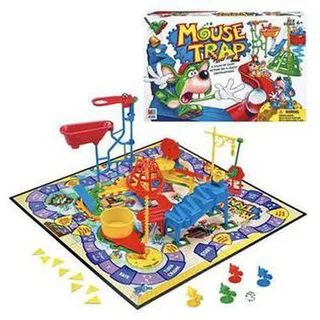
\includegraphics[width=0.4\textwidth]{figs/mouseTrap.png}
    \caption{Mouse Trap game (replace w/ system diagram)}
    \label{fig:sysDiagram}
\end{figure}


\subsection{System Transfer Function}
The open loop transfer function was found to be 
\begin{equation}
    P(s) = \frac{1}{s^2 + 2 \zeta \omega_n s + \omega_n^2}
\end{equation}
See \autoref{apx:sys_model_derivation} for derivation.

\subsection{Transient Response}

pole calculations and transient response statistics

\subsection{System Tracking Error}

under X standard input, the system provides an X steady-state error

(type calculation or direct computation)

include figure of matlab response

\subsection{Frequency Response}
Include bode plot of open loop response

identify important characteristics


%% Feedback Controller Design
\section{Feedback Controller Design}


TODO: include all the things


%% System Implimentation and Simulation
\section{System Implementation and Simulation}



TODO: include all the things



%% Conclusion
\section{Conclusion}
The conclusion goes here.

What did you learn by doing this project? 
What did you learn in this course?


\appendices

\section{Derivation of System Model}
\label{apx:sys_model_derivation}

\begin{align}
    u(t) &= \dv{t^2} x + 2 \zeta \omega_n \dv{t} x + \omega_n^2 x\\
    U(s) &= s^2 X(s) + 2 \zeta \omega_n s X(s) + \omega_n^2 X(s)\\
    \frac{X(s)}{U(s)} &= \frac{1}{s^2 + 2\zeta \omega_n s + \omega_n^2}
\end{align}

And any additional equations...

% if you want by leaving the argument blank
\section{}
Appendix two text goes here.


% use section* for acknowledgment
\section*{Acknowledgment}


The authors would like to thank...


% -----------------------------------------------------
% References
% -----------------------------------------------------
\bibliography{refs}{} 
\bibliographystyle{IEEEtran}







\end{document}